% !TeX program = xelatex
\documentclass[a4paper,10pt]{article}

% ============================================================================
% ១. កញ្ចប់បណ្ណាល័យ និងការកំណត់ទំព័រ (Packages & Page Setup — តាមគំរូ ls_plan.tex)
% ============================================================================
\usepackage[a4paper, left=0.95cm, right=0.95cm, top=0.85cm, bottom=0.92cm, footskip=0.52cm]{geometry}
\usepackage{amsmath}
\usepackage{unicode-math}
\usepackage{fontspec}
\usepackage{longtable, array, multirow, colortbl}
\usepackage[table]{xcolor}
\usepackage{enumitem}
\usepackage{pifont}
\usepackage{fancyhdr}
\usepackage{tikz}
\usetikzlibrary{calc, arrows.meta, decorations.pathreplacing, patterns, positioning, babel}

\makeatletter
\let\@expl@@@mark@update@singlecol@structures@@\relax
\makeatother

% --- ប្រព័ន្ធស្វែងរកទីតាំងពុម្ពអក្សរស្វ័យប្រវត្តិ (Windows Local + Cloud Repo fonts/) ---
\providecommand{\NGSFindFonts}{%
  \IfFileExists{C:/Windows/Fonts/cambria.ttc}{%
    \def\NGSSysPath{C:/Windows/Fonts/}%
    \def\NGSUserPath{C:/Users/KIT/AppData/Local/Microsoft/Windows/Fonts/}%
  }{%
    \IfFileExists{./fonts/KhmerOSsiemreap.ttf}{\def\NGSSysPath{./fonts/}\def\NGSUserPath{./fonts/}}{%
    \IfFileExists{../fonts/KhmerOSsiemreap.ttf}{\def\NGSSysPath{../fonts/}\def\NGSUserPath{../fonts/}}{%
    \IfFileExists{../../fonts/KhmerOSsiemreap.ttf}{\def\NGSSysPath{../../fonts/}\def\NGSUserPath{../../fonts/}}{%
    \IfFileExists{../../../fonts/KhmerOSsiemreap.ttf}{\def\NGSSysPath{../../../fonts/}\def\NGSUserPath{../../../fonts/}}{%
    \IfFileExists{../../../../fonts/KhmerOSsiemreap.ttf}{\def\NGSSysPath{../../../../fonts/}\def\NGSUserPath{../../../../fonts/}}{%
    \IfFileExists{../../../../../fonts/KhmerOSsiemreap.ttf}{\def\NGSSysPath{../../../../../fonts/}\def\NGSUserPath{../../../../../fonts/}}{%
    \IfFileExists{../../../../../../fonts/KhmerOSsiemreap.ttf}{\def\NGSSysPath{../../../../../../fonts/}\def\NGSUserPath{../../../../../../fonts/}}{%
      \def\NGSSysPath{../../../../../../../fonts/}\def\NGSUserPath{../../../../../../../fonts/}%
    }}}}}}}%
  }%
}
\NGSFindFonts

% ============================================================================
% ២. កំណត់ពុម្ពអក្សរ (Fonts — តាមគំរូ ls_plan.tex)
% ============================================================================
\setmathfont[Path={\NGSSysPath}, FontIndex=1, Scale=1.02]{cambria.ttc}
\defaultfontfeatures{Ligatures=TeX}

\setmainfont[
  Path={\NGSUserPath},
  Extension=.ttf,
  Script=Khmer,
  BoldFont={KhmerOSsiemreap},
  BoldFeatures={FakeBold=1.8},
  ItalicFont={KhmerOSsiemreap},
  ItalicFeatures={FakeSlant=0.25},
  BoldItalicFont={KhmerOSsiemreap},
  BoldItalicFeatures={FakeBold=1.8, FakeSlant=0.25}
]{KhmerOSsiemreap}

\newfontfamily\muol[Path={\NGSUserPath}, Extension=.ttf, Script=Khmer]{KhmerOSmuollight}
\newfontfamily\Tacteing[Path={\NGSUserPath}, Extension=.TTF]{TACTENG}
\newfontfamily\TimesEn[Path={\NGSSysPath}, Extension=.ttf, BoldFont={timesbd}, ItalicFont={timesi}, BoldItalicFont={timesbi}]{times}
\newfontfamily\CalibriFont[Path={\NGSSysPath}, Extension=.ttf]{calibri}
\newfontfamily\CourierCirc[Path={\NGSSysPath}, Extension=.ttf]{cour}

\XeTeXlinebreaklocale "km"
\XeTeXlinebreakskip = 0pt plus 1pt minus 0.1pt

% ============================================================================
% ៣. ពណ៌ និងការតុបតែង (Colors & Styles)
% ============================================================================
\definecolor{stepbg}{HTML}{D9D9D9}
\definecolor{headgray}{HTML}{E6E6E6}
\definecolor{emphred}{HTML}{C00000}

\pagestyle{fancy}
\fancyhf{}
\renewcommand{\headrulewidth}{0pt}
\fancyfoot[R]{\CalibriFont\fontsize{9pt}{11pt}\selectfont\thepage}

\setlength{\parindent}{0pt}
\setlength{\parskip}{0pt}
\setlength{\tabcolsep}{4.5pt}
\setlength{\LTpre}{2pt}
\setlength{\LTpost}{2pt}

\newcolumntype{L}[1]{>{\raggedright\arraybackslash}p{#1}}
\newcolumntype{C}[1]{>{\centering\arraybackslash}p{#1}}

% ============================================================================
% ៤. ពាក្យបញ្ជាជំនួយ (Helper Macros)
% ============================================================================
\newcommand{\en}[1]{{\TimesEn #1}}
\newcommand{\enbf}[1]{{\TimesEn\bfseries #1}}
\newcommand{\khmflourish}{{\Tacteing\fontsize{15pt}{15pt}\selectfont 3}}
\newcommand{\wcirc}{{\CourierCirc\fontsize{9.5pt}{11pt}\selectfont o}}
\newcommand{\ditem}{{\fontsize{7.5pt}{10pt}\selectfont\ding{117}}\ }
\newcommand{\fiveE}[1]{\textcolor{emphred}{\CalibriFont\bfseries #1}}
\newcommand{\redsub}[1]{\textcolor{emphred}{#1}}
\newcommand{\timenote}[1]{\textcolor{emphred}{\textit{#1}}}
\newcommand{\stepheader}[1]{\multicolumn{3}{|c|}{\cellcolor{stepbg}\muol #1} \\ \hline}
\newcommand{\cfig}[1]{{\centering\vspace{3pt}#1\vspace{3pt}\par}}
\newcommand{\cnum}[1]{\mbox{\fontsize{10.5pt}{12pt}\selectfont\ding{\numexpr181+#1\relax}}}
\newcommand{\unit}[1]{\,\text{\en{#1}}}
\newcommand{\riel}{\,\text{៛}}
\newcommand{\graybox}[1]{\colorbox{headgray}{\strut #1}}

% ============================================================================
% ៥. រូបភាព TikZ ស-ខ្មៅ សម្រាប់បង្រៀនលើក្ដារខៀន និងសន្លឹកកិច្ចការ (B&W Diagrams)
% ============================================================================

% ១. E1 Engage: អន្ទាក់សម្រួលតួឆ្លងសញ្ញាបូកក្នុង (3x^2+4x)/(9x^2-16) (ទំ.៧៧)
\newcommand{\figEngageRATSixTwo}{%
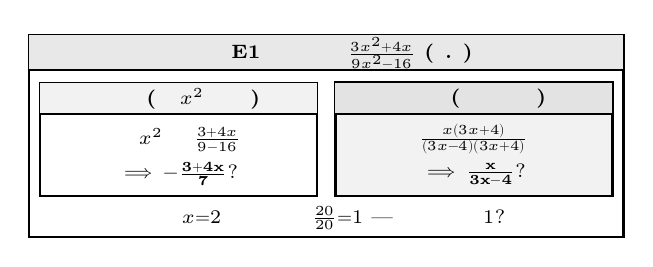
\begin{tikzpicture}[x=1cm, y=1cm, every node/.style={font=\scriptsize, text=black}]
  \draw[black, line width=0.9pt] (0,0) rectangle (7.55,2.56);
  \fill[gray!18] (0,2.12) rectangle (7.55,2.56);
  \draw[black, line width=0.6pt] (0,2.12) -- (7.55,2.12);
  \node at (3.775,2.34) {\textbf{បេសកកម្ម \en{E1}៖ សម្រួលកន្សោម $\tfrac{3x^2 + 4x}{9x^2 - 16}$ (ទំ.៧៧)}};

  % Student A
  \draw[black, line width=0.8pt] (0.14,0.52) rectangle (3.66,1.96);
  \fill[gray!10] (0.14,1.56) rectangle (3.66,1.96);
  \draw[black, line width=0.5pt] (0.14,1.56) -- (3.66,1.56);
  \node at (1.90,1.76) {\textbf{សិស្ស ក (ឈូត $x^2$ ឆ្លងបូក)}};
  \node at (1.90,1.24) {ឈូត $x^2$ បាន $\tfrac{3 + 4x}{9 - 16}$};
  \node at (1.90,0.80) {$\implies \mathbf{-\tfrac{3 + 4x}{7}}$?};

  % Student B
  \draw[black, line width=0.95pt, fill=gray!10] (3.89,0.52) rectangle (7.41,1.96);
  \fill[gray!22] (3.89,1.56) rectangle (7.41,1.96);
  \draw[black, line width=0.55pt] (3.89,1.56) -- (7.41,1.56);
  \node at (5.65,1.76) {\textbf{សិស្ស ខ (ដាក់ជាកត្តាសិន)}};
  \node at (5.65,1.24) {$\tfrac{x(3x+4)}{(3x-4)(3x+4)}$};
  \node at (5.65,0.80) {$\implies \mathbf{\tfrac{x}{3x - 4}}$?};

  \node at (3.775,0.24) {\textbf{តេស្ត $x{=}2$៖} កន្សោមដើមស្មើ $\tfrac{20}{20}{=}1$ — តើចម្លើយណាស្មើ $1$?};
\end{tikzpicture}}

% ២. E2 Explore: សម្រួលតាមកត្តារួម និងកត្តាផ្ទុយ 1-x = -(x-1) (ទំ.៧៦--៧៧)
\newcommand{\figExploreRATSixTwo}{%
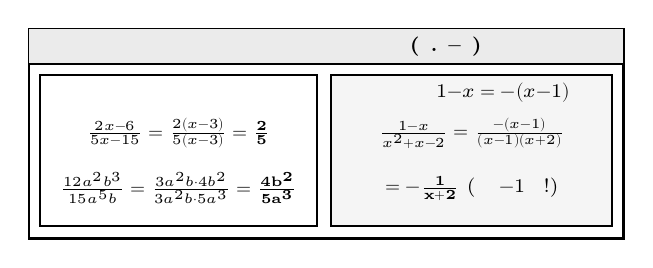
\begin{tikzpicture}[x=1cm, y=1cm, every node/.style={font=\scriptsize, text=black}]
  \draw[black, line width=0.9pt] (0,0) rectangle (7.55,2.66);
  \fill[gray!16] (0,2.22) rectangle (7.55,2.66);
  \draw[black, line width=0.6pt] (0,2.22) -- (7.55,2.22);
  \node at (3.775,2.44) {\textbf{ការដាក់ជាផលគុណកត្តា និងកត្តាផ្ទុយមុនសម្រួល (ទំ.៧៦--៧៧)}};

  % Left: GCF & Monomials
  \draw[black, line width=0.8pt] (0.14,0.16) rectangle (3.66,2.08);
  \node at (1.90,1.86) {\textbf{កត្តារួម និងឯកធា}};
  \node at (1.90,1.34) {$\tfrac{2x-6}{5x-15} = \tfrac{2(x-3)}{5(x-3)} = \mathbf{\tfrac{2}{5}}$};
  \node at (1.90,0.64) {$\tfrac{12a^2b^3}{15a^5b} = \tfrac{3a^2b\cdot 4b^2}{3a^2b\cdot 5a^3} = \mathbf{\tfrac{4b^2}{5a^3}}$};

  % Right: Opposite factor
  \draw[black, line width=0.8pt, fill=gray!8] (3.84,0.16) rectangle (7.41,2.08);
  \node at (5.625,1.86) {\textbf{កត្តាផ្ទុយ $1{-}x = -(x{-}1)$}};
  \node at (5.625,1.34) {$\tfrac{1 - x}{x^2 + x - 2} = \tfrac{-(x - 1)}{(x - 1)(x + 2)}$};
  \node at (5.625,0.64) {$= \mathbf{-\tfrac{1}{x + 2}}$ (សល់ $-1$ លើ!)};
\end{tikzpicture}}

% ៣. E3 Explain: វិធាន AK/BK = A/B និងកត្តាផ្ទុយ (ទំ.៧៧)
\newcommand{\figRuleRATSixTwo}{%
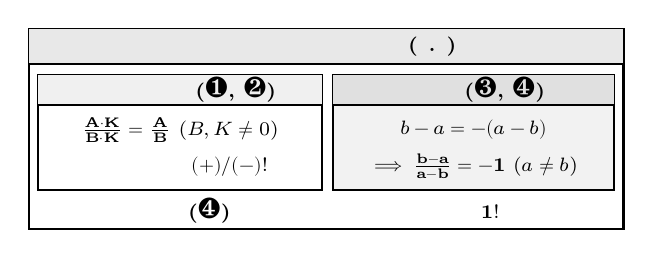
\begin{tikzpicture}[x=1cm, y=1cm, every node/.style={font=\scriptsize, text=black}]
  \draw[black, line width=0.9pt] (0,0) rectangle (7.55,2.54);
  \fill[gray!18] (0,2.10) rectangle (7.55,2.54);
  \draw[black, line width=0.6pt] (0,2.10) -- (7.55,2.10);
  \node at (3.775,2.32) {\textbf{វិធានសម្រួលកន្សោមសនិទាន និងកត្តាផ្ទុយ (ទំ.៧៧)}};

  % Left: Main rule
  \draw[black, line width=0.8pt] (0.12,0.50) rectangle (3.72,1.96);
  \fill[gray!12] (0.12,1.58) rectangle (3.72,1.96);
  \draw[black, line width=0.55pt] (0.12,1.58) -- (3.72,1.58);
  \node at (1.92,1.77) {\textbf{ក្បួនសម្រួលកត្តារួម (\cnum{1}, \cnum{2})}};
  \node at (1.92,1.26) {$\mathbf{\tfrac{A \cdot K}{B \cdot K} = \tfrac{A}{B}}$ ($B, K \neq 0$)};
  \node at (1.92,0.80) {ហាមឈូតតួឆ្លងសញ្ញា $(+)/(-)$!};

  % Right: Opposite factors
  \draw[black, line width=0.95pt, fill=gray!10] (3.86,0.50) rectangle (7.43,1.96);
  \fill[gray!24] (3.86,1.58) rectangle (7.43,1.96);
  \draw[black, line width=0.6pt] (3.86,1.58) -- (7.43,1.58);
  \node at (5.645,1.77) {\textbf{កត្តាផ្ទុយ (\cnum{3}, \cnum{4})}};
  \node at (5.645,1.26) {$b - a = -(a - b)$};
  \node at (5.645,0.80) {$\implies \mathbf{\tfrac{b - a}{a - b} = -1}$ ($a \neq b$)};

  \node at (3.775,0.24) {\textbf{ចំណាំ (\cnum{4})៖} បើកត្តាទាំងអស់នៅភាគយកសម្រួលអស់ ត្រូវសល់លេខ $\mathbf{1}$!};
\end{tikzpicture}}

% ៤. E4 Elaborate: លំហាត់គំរូ ១ និងរង្វង់ចារឹកក្នុងការេ ទំ.៧៨
\newcommand{\figElaborateRATSixTwo}{%
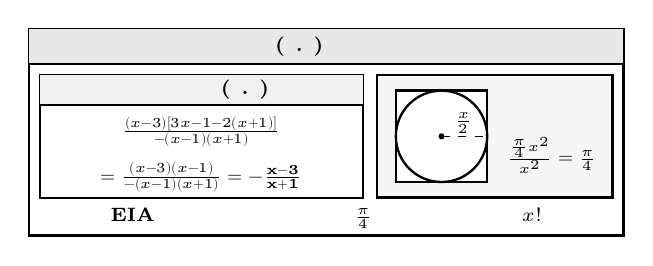
\begin{tikzpicture}[x=1cm, y=1cm, every node/.style={font=\scriptsize, text=black}]
  \draw[black, line width=0.9pt] (0,0) rectangle (7.55,2.62);
  \fill[gray!18] (0,2.18) rectangle (7.55,2.62);
  \draw[black, line width=0.6pt] (0,2.18) -- (7.55,2.18);
  \node at (3.775,2.40) {\textbf{លំហាត់គំរូទី ១ និងទី ២ (ទំ.៧៨)៖ កត្តារួម និងរង្វង់ចារឹកក្នុងការេ}};

  % Left: Worked example 1
  \draw[black, line width=0.8pt] (0.14,0.48) rectangle (4.24,2.04);
  \fill[gray!12] (0.14,1.66) rectangle (4.24,2.04);
  \draw[black, line width=0.55pt] (0.14,1.66) -- (4.24,1.66);
  \node at (2.19,1.85) {\textbf{លំហាត់គំរូទី ១ (ទំ.៧៨)}};
  \node at (2.19,1.32) {$\tfrac{(x-3)[3x-1-2(x+1)]}{-(x-1)(x+1)}$};
  \node at (2.19,0.74) {$= \tfrac{(x-3)(x-1)}{-(x-1)(x+1)} = \mathbf{-\tfrac{x-3}{x+1}}$};

  % Right: Inscribed circle in square (true B&W geometry!)
  \draw[black, line width=0.95pt, fill=gray!8] (4.42,0.48) rectangle (7.41,2.04);
  \draw[black, line width=0.85pt, fill=white] (4.66,0.68) rectangle (5.82,1.84);
  \draw[black, line width=0.85pt] (5.24,1.26) circle (0.58);
  \fill (5.24,1.26) circle (1.1pt);
  \draw[black, dashed, line width=0.6pt] (5.24,1.26) -- (5.82,1.26);
  \node at (5.52,1.43) {$\tfrac{x}{2}$};
  \node at (6.64,1.56) {\textbf{គំរូទី ២}};
  \node at (6.64,1.02) {$\tfrac{\frac{\pi}{4}x^2}{x^2} = \tfrac{\pi}{4}$};

  \node at (3.775,0.22) {\textbf{\en{EIA}៖} ផលធៀបផ្ទៃរង្វង់ចារឹកក្នុងការេស្មើ $\tfrac{\pi}{4}$ មិនអាស្រ័យនឹងរង្វាស់ជ្រុង $x$!};
\end{tikzpicture}}

% ៥. E5 Evaluate: ជម្រើសវិនិច្ឆ័យ A-D សម្រួល (x^2 - 9)/(3 - x)
\newcommand{\figExitRATSixTwo}{%
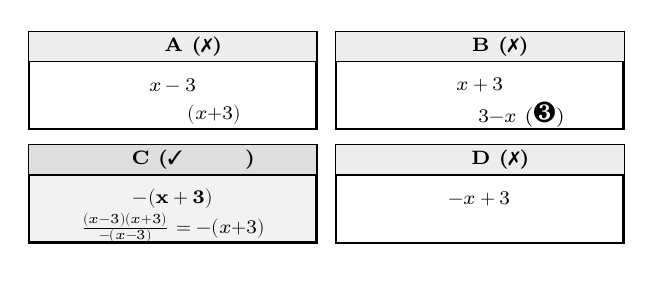
\begin{tikzpicture}[x=1cm, y=1cm, every node/.style={font=\scriptsize, text=black}]
  % Choice A
  \draw[black, line width=0.8pt] (0,1.44) rectangle (3.65,2.68);
  \fill[gray!14] (0,2.30) rectangle (3.65,2.68);
  \draw[black, line width=0.5pt] (0,2.30) -- (3.65,2.30);
  \node at (1.825,2.49) {\textbf{ជម្រើស \en{A} (\ding{55})}};
  \node at (1.825,2.00) {$x - 3$};
  \node at (1.825,1.62) {សម្រួលខុសកត្តា $(x{+}3)$};

  % Choice B
  \draw[black, line width=0.8pt] (3.90,1.44) rectangle (7.55,2.68);
  \fill[gray!14] (3.90,2.30) rectangle (7.55,2.68);
  \draw[black, line width=0.5pt] (3.90,2.30) -- (7.55,2.30);
  \node at (5.725,2.49) {\textbf{ជម្រើស \en{B} (\ding{55})}};
  \node at (5.725,2.00) {$x + 3$};
  \node at (5.725,1.62) {ភ្លេចសញ្ញាដកនៃ $3{-}x$ (\cnum{3})};

  % Choice C (Correct)
  \draw[black, line width=1.0pt, fill=gray!10] (0,0) rectangle (3.65,1.24);
  \fill[gray!26] (0,0.86) rectangle (3.65,1.24);
  \draw[black, line width=0.55pt] (0,0.86) -- (3.65,0.86);
  \node at (1.825,1.05) {\textbf{ជម្រើស \en{C} (\ding{51} ត្រឹមត្រូវ)}};
  \node at (1.825,0.56) {$\mathbf{-(x + 3)}$};
  \node at (1.825,0.18) {$\tfrac{(x-3)(x+3)}{-(x-3)} = -(x{+}3)$};

  % Choice D
  \draw[black, line width=0.8pt] (3.90,0) rectangle (7.55,1.24);
  \fill[gray!14] (3.90,0.86) rectangle (7.55,1.24);
  \draw[black, line width=0.5pt] (3.90,0.86) -- (7.55,0.86);
  \node at (5.725,1.05) {\textbf{ជម្រើស \en{D} (\ding{55})}};
  \node at (5.725,0.56) {$-x + 3$};
  \node at (5.725,0.18) {មិនបានគុណដកចូលវង់ក្រចក};
\end{tikzpicture}}

% ============================================================================
% ៦. ចាប់ផ្ដើមឯកសារ (Document Body)
% ============================================================================
\begin{document}
\fontsize{10pt}{15.2pt}\selectfont

% --- ក្បាលរដ្ឋបាល (Administrative Header) ---
\begin{center}
  {\muol\fontsize{11pt}{16pt}\selectfont ព្រះរាជាណាចក្រកម្ពុជា}\\[2pt]
  {\muol\fontsize{11pt}{16pt}\selectfont ជាតិ សាសនា ព្រះមហាក្សត្រ}\\[-2pt]
  \khmflourish
\end{center}
\vspace{-4pt}

{\muol\fontsize{10pt}{15pt}\selectfont
មន្ទីរអប់រំ យុវជន និងកីឡា ខេត្តកំពង់ធំ\\
ការិយាល័យអប់រំ យុវជន និងកីឡា ស្រុកកំពង់ស្វាយ\\
អនុវិទ្យាល័យព្រះក្រសាំង}

\vspace{2pt}
\begin{center}
  {\muol\fontsize{12pt}{18pt}\selectfont កិច្ចតែងការបង្រៀន}
\end{center}
\vspace{1pt}

% --- ព័ត៌មានទូទៅ (General Metadata) ---
\begin{tabular}{@{}p{1.85cm}p{3.25cm}@{\hspace{4pt}:\hspace{6pt}}p{12.65cm}@{}}
  & - \quad មុខវិជ្ជា          & គណិតវិទ្យា ថ្នាក់ទី៨ (ពីជគណិត) \\
  & - \quad ចំណងជើងមេរៀន & មេរៀនទី៦៖ កន្សោមសនិទាន \\
  & - \quad ចំណងជើងរង      & ៣. ការសម្រួលកន្សោមសនិទាន \\
  & - \quad រយៈពេល             & ១ ម៉ោងសិក្សា (៥០ នាទី) \\
  & - \quad បង្រៀនដោយ         & ហុក ប៊ុនថែន \\
  & - \quad កាលបរិច្ឆេទ        & ថ្ងៃអង្គារ ទី១៥ ខែធ្នូ ឆ្នាំ២០២៦ \\
\end{tabular}

\vspace{4pt}

% --- I. វត្ថុបំណង ---
{\muol\enbf{I.} វត្ថុបំណង}\par\vspace{2pt}
\begin{tabular}{@{}p{0.55cm}p{2.55cm}@{\hspace{2pt}:\hspace{6pt}}L{15.4cm}@{}}
  & \wcirc វិជ្ជាសម្បទា   & សិស្សប្រាប់បាននូវវិធានសម្រួលកន្សោមសនិទាន $\tfrac{AK}{BK} = \tfrac{A}{B}$ ($K \neq 0$) និងលក្ខណៈកត្តាផ្ទុយ $b - a = -(a - b)$ បានត្រឹមត្រូវ (ទំ.៧៦–៧៨) ។ \\[2pt]
  & \wcirc បំណិនសម្បទា & សិស្សដាក់ភាគយកនិងភាគបែងជាផលគុណកត្តា រួចសម្រួលកន្សោមសនិទានលើសន្លឹកកិច្ចការបានត្រឹមត្រូវតាមជំហាន ។ \\[2pt]
  & \wcirc ចរិយាសម្បទា  & សិស្សមានទម្លាប់ដាក់កន្សោមជាផលគុណកត្តាមុននឹងសម្រួល និងជៀសវាងការឈូតតួឆ្លងសញ្ញាបូកឬដកប្រកបដោយភាពម៉ត់ចត់ ។ \\
\end{tabular}

\vspace{3pt}

% --- II. សម្ភារៈឧបទេស (Zero-LCD & Fill-In Worksheet Context) ---
{\muol\enbf{II.} សម្ភារៈឧបទេស}\par\vspace{2pt}
\hspace*{0.55cm}$\bullet$ សៀវភៅសិក្សាគោលថ្នាក់ទី៨ (ទំ.៧៦--៧៨, ៨៥) ក្ដារខៀន ដីស/ហ្វឺត បន្ទាត់ត្រង់ និង\textbf{សន្លឹកកិច្ចការសិស្សបំពេញចន្លោះ ស-ខ្មៅ} (កូដ \en{RAT62} ទំព័រ ១--២ សម្រាប់សិស្ស និងទំព័រ ៣ ប្លង់ក្ដារខៀន/ចម្លើយគ្រូ — គ្មានប្រើ \en{LCD})

\vspace{3pt}

% --- III. វិធីសាស្រ្តបង្រៀន ---
{\muol\enbf{III.} វិធីសាស្រ្តបង្រៀន}\par\vspace{2pt}
\begin{tabular}{@{}p{0.55cm}p{2.55cm}@{\hspace{2pt}:\hspace{6pt}}L{15.4cm}@{}}
  & $\bullet$ គោលវិធី      & សិស្សមជ្ឈមណ្ឌល (សន្លឹកកិច្ចការបំពេញចន្លោះជាគោល + ការពិភាក្សាជាក្រុមតូច ៣ នាក់) \\
  & $\bullet$ យុទ្ធវិធីបង្រៀន & គំរូស្ថាបនានិយម \en{5Es} រួមបញ្ចូល \textit{ការវិភាគលំហាត់គំរូខុស (\en{Erroneous Examples})} និង \textit{ការចាក់សោកញ្ចប់កត្តា} \\
\end{tabular}

\vspace{4pt}

% --- IV. ដំណើរការបង្រៀន (50-Minute 5E Flow) ---
{\muol\enbf{IV.} ដំណើរការបង្រៀន}\par\vspace{1pt}

\renewcommand{\arraystretch}{1.15}
\begin{longtable}{|L{5.50cm}|L{7.90cm}|L{4.80cm}|}
\hline
\multicolumn{1}{|c|}{\cellcolor{headgray}\muol សកម្មភាពគ្រូ} &
\multicolumn{1}{c|}{\cellcolor{headgray}\muol ខ្លឹមសារមេរៀន} &
\multicolumn{1}{c|}{\cellcolor{headgray}\muol សកម្មភាពសិស្ស} \\[2pt]
\hline
\endfirsthead

\hline
\multicolumn{1}{|c|}{\cellcolor{headgray}\muol សកម្មភាពគ្រូ} &
\multicolumn{1}{c|}{\cellcolor{headgray}\muol ខ្លឹមសារមេរៀន} &
\multicolumn{1}{c|}{\cellcolor{headgray}\muol សកម្មភាពសិស្ស} \\[2pt]
\hline
\endhead

\hline
\endfoot

% ==================== ជំហានទី១ (2min) ====================
\stepheader{ជំហានទី១ \enbf{(}រដ្ឋបាលថ្នាក់\enbf{)}}
$\bullet$ ពិនិត្យវត្តមាន អនាម័យ និងសណ្ដាប់ធ្នាប់ថ្នាក់រៀន \par
$\bullet$ រៀបចំក្រុមតូច ៣ នាក់ និងចែក\textbf{សន្លឹកកិច្ចការសិស្ស} (\en{RAT62} ទំព័រ ១–២)
&
$\bullet$ រដ្ឋបាលថ្នាក់ អនាម័យ និងវិន័យសិក្សា \par
$\bullet$ ចែកសន្លឹកកិច្ចការម្នាក់ ១ សន្លឹក សម្រាប់បំពេញតាមដំណាក់កាល \en{E1--E5}
&
$\circ$ ប្រធានថ្នាក់រាយការណ៍វត្តមានសិស្ស \par
$\circ$ ទទួលសន្លឹកកិច្ចការ សរសេរឈ្មោះ និងអង្គុយតាមក្រុម ៣ នាក់ \\
\hline

% ==================== ជំហានទី២ (9min: កំណែ ≤3m + រំលឹក 3m + E1 3m) ====================
\stepheader{ជំហានទី២ \enbf{(}កិច្ចការផ្ទះ \enbf{+} ទំនាក់ទំនងមេរៀនថ្មី\enbf{)}}
\ditem \textbf{កំណែកិច្ចការផ្ទះ (\enbf{$\le$ 3 min})} \par
$\bullet$ ហៅសិស្ស ២ នាក់ឡើងកែលំហាត់ទំ.៨៥ \en{\#1} ខ និង \en{\#2} ឃ, \en{\#4} គ លើក្ដារខៀន
&
\hspace*{0.15cm}\redsub{កំណែកិច្ចការផ្ទះ (ទំ.៨៥ លេខ ១, ២, ៣, ៤)} \par
$\bullet$ \textbf{\en{\#1} ខ៖} ចំពោះ $a = -2$ បាន $\mathbf{0}$; ចំពោះ $a = -\tfrac{1}{2}$ និង $a = 1$ \textbf{គ្មានន័យ} \par
$\bullet$ \textbf{\en{\#2} ឃ, \en{\#3} គ, \en{\#4} គ៖} \en{\#2} ឃ) $x \neq \pm 4$; \ \en{\#3} គ) $a = 0, 2$; \ \en{\#4} គ) $x = 1, 5$
&
$\circ$ ផ្ទៀងចម្លើយ និងកែតម្រូវចូលសៀវភៅកិច្ចការផ្ទះ \\[3pt]

\ditem \textbf{រំលឹកមេរៀនទាក់ទង (\enbf{3min})} \par
$\bullet$ សួរ៖ «តើគេសម្រួលប្រភាគ $\tfrac{18}{24}$ ដោយវិធីណា? ចុះដាក់ $9x^2 - 16$ និង $x^2 + x - 2$ ជាផលគុណកត្តាបានអ្វី?»
&
\hspace*{0.15cm}\redsub{រំលឹកការសម្រួលប្រភាគ និងការដាក់ជាផលគុណកត្តា} \par
$\bullet$ សម្រួលប្រភាគ៖ $\dfrac{18}{24} = \dfrac{3 \times 6}{4 \times 6} = \dfrac{3}{4}$ (ចែកនឹងកត្តារួម $6$) \par
$\bullet$ $9x^2 - 16 = (3x - 4)(3x + 4)$; \quad $x^2 + x - 2 = (x - 1)(x + 2)$
&
$\circ$ ឆ្លើយ៖ «ចែកនឹងកត្តារួម $6$ បាន $\tfrac{3}{4}$ និងបំបែកជាផលគុណកត្តា!» \\[3pt]

\fiveE{E1 - Engage (3min)} \timenote{(កុំទាន់ផ្តល់ចម្លើយ)} \par
\ditem \textbf{បេសកកម្មអន្ទាក់ឈូតតួឆ្លងសញ្ញាបូក (សន្លឹកកិច្ចការ \en{E1})} \par
$\bullet$ ឱ្យសិស្សអានប្រអប់ \en{E1} ពិនិត្យការសម្រួល $\dfrac{3x^2 + 4x}{9x^2 - 16}$ (ទំ.៧៧) ដោយជំនួស $x = 2$
&
\redsub{បេសកកម្ម \en{E1}៖ សម្រួល $\dfrac{3x^2 + 4x}{9x^2 - 16}$ តាមវិធីណាទើបត្រូវ? (ទំ.៧៧)} \par
$\bullet$ \textbf{សិស្ស ក} ឈូត $x^2$ ឆ្លងសញ្ញាបូក-ដក បាន $-\dfrac{3 + 4x}{7}$! \par
$\bullet$ \textbf{សិស្ស ខ} ដាក់ជាផលគុណកត្តាសិន បាន $\dfrac{x}{3x - 4}$! តេស្ត $x = 2$ មើល៍!
&
$\circ$ ជំនួស $x = 2$ ពិភាក្សាជាគូ និងគូស \ding{51} ក្នុងប្រអប់ \en{E1} \\[3pt]

&
\cfig{\figEngageRATSixTwo}
& \\
\hline

% ==================== ជំហានទី៣ (17min: E2 11m + E3 6m) ====================
\stepheader{ជំហានទី៣ \enbf{(}ខ្លឹមសារមេរៀនថ្មី\enbf{)}}
\fiveE{E2 - Explore (11min)} \par
$\bullet$ សរសេរចំណងជើងរង \textbf{៣. ការសម្រួលកន្សោមសនិទាន} លើក្ដារខៀន \par
\ditem \textbf{សកម្មភាព ១៖ សម្រួលតាមកត្តារួម និងឯកធា (ទំ.៧៦–៧៧, \enbf{5min}, \en{E2-A})} \par
$\bullet$ ឱ្យសិស្សបំពេញឧទាហរណ៍ទី ១ និងទី ២ (ទំ.៧៦–៧៧) លើ \en{E2-A}
&
៣. ការសម្រួលកន្សោមសនិទាន (ទំ.៧៦–៧៧) \par
$\bullet$ \textbf{ឧទាហរណ៍ទី ១៖} $\dfrac{2x - 6}{5x - 15} = \dfrac{2(x - 3)}{5(x - 3)} = \mathbf{\dfrac{2}{5}}$ (សម្រួលកត្តារួម $x - 3 \neq 0$) \par
$\bullet$ \textbf{ឧទាហរណ៍ទី ២៖} $\dfrac{12a^2b^3}{15a^5b} = \dfrac{3a^2b \cdot 4b^2}{3a^2b \cdot 5a^3} = \mathbf{\dfrac{4b^2}{5a^3}}$ (សម្រួល $3a^2b \neq 0$)
&
$\circ$ ដាក់ជាផលគុណកត្តា និងសម្រួលកត្តារួមលើ \en{E2-A} \\[3pt]

\ditem \textbf{សកម្មភាព ២៖ សមភាពសំខាន់ៗ និងកត្តាផ្ទុយ (ទំ.៧៧, \enbf{6min}, \en{E2-B})} \par
$\bullet$ ឱ្យសិស្សបំពេញឧទាហរណ៍ទី ៣ និងឧទាហរណ៍ទី ៤ ($1 - x = -(x - 1)$) លើ \en{E2-B}
&
ការប្រើសមភាពសំខាន់ៗ និងកត្តាផ្ទុយ (ទំ.៧៧) \par
$\bullet$ \textbf{ឧទាហរណ៍ទី ៣៖} $\dfrac{3x^2 + 4x}{9x^2 - 16} = \dfrac{x(3x + 4)}{(3x - 4)(3x + 4)} = \mathbf{\dfrac{x}{3x - 4}}$ \par
$\bullet$ \textbf{ឧទាហរណ៍ទី ៤៖} $\dfrac{1 - x}{x^2 + x - 2} = \dfrac{-(x - 1)}{(x - 1)(x + 2)} = \mathbf{-\dfrac{1}{x + 2}}$
&
$\circ$ បំបែកកត្តា និងទាញសញ្ញាដកពី $1 - x = -(x - 1)$ លើ \en{E2-B} \\[3pt]

&
\cfig{\figExploreRATSixTwo}
& \\[3pt]

% --- E3 Explain (6min) ---
\fiveE{E3 - Explain (6min)} \par
$\bullet$ ដឹកនាំសិស្សសង្ខេបវិធានសម្រួលកន្សោមសនិទាន និងកត្តាផ្ទុយ (ទំ.៧៧)
&
$\bullet$ \textbf{ជាទូទៅ (ទំ.៧៧)៖} ដើម្បីសម្រួលកន្សោមសនិទាន គេត្រូវ\textbf{ដាក់ភាគយកនិងភាគបែងជាផលគុណកត្តា} រួចចែកនឹងកត្តារួមខុសពីសូន្យ៖ \par
\hspace*{0.15cm}– ក្បួនគ្រឹះ៖ $\graybox{$\dfrac{AK}{BK} = \dfrac{A}{B}$}$ ($B, K \neq 0$);\quad កត្តាផ្ទុយ៖ $\graybox{$\dfrac{b - a}{a - b} = -1$}$ ($a \neq b$)
&
$\circ$ បំពេញប្រអប់វិធានជាទូទៅលើសន្លឹកកិច្ចការ \en{E3} \\[3pt]

$\bullet$ ភ្ជាប់\textbf{ធនាគារហេតុផល \cnum{1}--\cnum{4}} លើក្ដារខៀន និងសន្លឹកកិច្ចការ
&
\textbf{ធនាគារហេតុផល (\en{Warrant Bank})៖} \par
\cnum{1} \textbf{ហាមឈូតតួឆ្លងបូក-ដក៖} ត្រូវដាក់ភាគយកនិងភាគបែងជាផលគុណកត្តាសិនមុននឹងសម្រួល \par
\cnum{2} \textbf{កត្តារួមខុសពីសូន្យ៖} ចែកភាគយកនិងភាគបែងនឹងកញ្ចប់កត្តារួម $K \neq 0$ ទាំងមូល
&
$\circ$ ផ្ទៀងលេខកូដ \cnum{1}--\cnum{2} លើសន្លឹកកិច្ចការ \\[3pt]

&
\cnum{3} \textbf{លក្ខណៈកត្តាផ្ទុយ៖} ទាញសញ្ញាដក $b - a = -(a - b)$ ដើម្បីបង្កើតកត្តារួម $(a - b)$
&
$\circ$ ផ្ទៀងលេខកូដ \cnum{3} លើសន្លឹកកិច្ចការ \\[3pt]

&
\cnum{4} \textbf{សល់លេខ $1$ មិនមែន $0$៖} បើកត្តាទាំងអស់នៅភាគយកសម្រួលអស់ ភាគយកនៅសល់លេខ $1$
&
$\circ$ ផ្ទៀងលេខកូដ \cnum{4} លើសន្លឹកកិច្ចការ \\[3pt]

&
\cfig{\figRuleRATSixTwo}
& \\
\hline

% ==================== ជំហានទី៤ (20min: E4 10m + E5 10m) ====================
\stepheader{ជំហានទី៤ \enbf{(}ពង្រីកចំណេះដឹង\enbf{)}}
\fiveE{E4 - Elaborate (10min)} \par
\ditem \textbf{លំហាត់គំរូទី ១–២ និងប្រតិបត្តិ ក, ខ (ទំ.៧៨)} \par
$\bullet$ ឱ្យសិស្សធ្វើលំហាត់គំរូទី ១, ទី ២ និងប្រតិបត្តិ ក, ខ (ទំ.៧៨) លើ \en{E4}
&
\textbf{លំហាត់គំរូពង្រីក (ទំ.៧៨)៖} \par
$\bullet$ \textbf{១) គំរូ ១៖} $\dfrac{(x-3)(3x-1)-(2x-6)(x+1)}{1-x^2} = \dfrac{(x-3)(x-1)}{-(x-1)(x+1)} = \graybox{$-\dfrac{x-3}{x+1}$}$ \par
$\bullet$ \textbf{២) គំរូ ២ (រង្វង់ចារឹកក្នុងការេជ្រុង $x$)៖} កាំ $\dfrac{x}{2} \implies$ ផលធៀបផ្ទៃក្រឡាគឺ $\dfrac{\frac{\pi}{4}x^2}{x^2} = \graybox{$\dfrac{\pi}{4}$}$ \par
$\bullet$ \textbf{៣) ប្រតិបត្តិ ក, ខ (ទំ.៧៨)៖} ក) $\dfrac{a-b}{b^2-a^2} = \mathbf{-\dfrac{1}{a+b}}$;\quad ខ) $\dfrac{(a-1)(5-a)}{(a+2)(5-a)} = \mathbf{\dfrac{a-1}{a+2}}$
&
$\circ$ ចាប់កត្តារួម ប្រើកត្តាផ្ទុយ និងសម្រួលលើ \en{E4} \\[3pt]

&
\cfig{\figElaborateRATSixTwo}
& \\[3pt]

$\bullet$ សួរសំណួរឆ្លុះបញ្ចាំង \textbf{\en{EIA Looking-Back}} (\enbf{1min})
&
\textbf{\en{EIA Looking-Back}៖} «ក្នុងប្រតិបត្តិ ក) $\dfrac{a-b}{b^2-a^2}$ ហេតុអ្វីក្រោយសម្រួល $(b-a)$ ចេញ ភាគយកនៅសល់ $-1$ មិនមែន $0$?» ($\to$ ព្រោះ $a - b = -1 \cdot (b - a)$ ការចែកកត្តាដូចគ្នាបាន $1$ \cnum{3}, \cnum{4}!)
&
$\circ$ ពន្យល់ថា $a-b = -(b-a)$ ពេលចែកនឹង $(b-a)$ បាន $-1$ \\[3pt]

% --- E5 Evaluate (10min) ---
\fiveE{E5 - Evaluate (10min)} \par
\ditem \textbf{ប្រតិបត្តិជាក្រុមតូច ៣ នាក់ (\enbf{4min}, សន្លឹកកិច្ចការ \en{E5})} \par
$\bullet$ ឱ្យសិស្សដោះស្រាយប្រតិបត្តិ គ, ឃ (ទំ.៧៨) និងទំ.៨៥ \en{\#5} ក, ឃ, ច
&
\textbf{លំហាត់ប្រតិបត្តិ (ទំ.៧៨ គ, ឃ និង ទំ.៨៥ \en{\#5})៖} \par
$\bullet$ \textbf{១) ប្រតិបត្តិ គ, ឃ (ទំ.៧៨)៖} គ) $\dfrac{x-y}{(x-y)(x+z)} = \mathbf{\dfrac{1}{x+z}}$; \quad ឃ) $\dfrac{3a(a-2)(a+1)}{6a(a-3)(a+1)} = \mathbf{\dfrac{a-2}{2(a-3)}}$ \par
$\bullet$ \textbf{២) ទំ.៨៥ \en{\#5} ក, ឃ, ច៖} ក) $\mathbf{\dfrac{2x}{y}}$; \quad ឃ) $\mathbf{\dfrac{1}{2a(x+3)}}$; \quad ច) $\dfrac{-(5x-1)(5x+1)}{5x-1} = \mathbf{-(5x+1)}$
&
$\circ$ សហការគ្នាដាក់ជាផលគុណកត្តា និងសម្រួលលើ \en{E5} \\[3pt]

$\bullet$ ឱ្យក្រុមសិស្សផ្ទៀងផ្ទាត់និងបិទ\textbf{បេសកកម្ម \en{E1}} (\enbf{2min})
&
$\bullet$ \textbf{បិទបេសកកម្ម \en{E1}៖} សិស្ស ខ ត្រឹមត្រូវ! ចំពោះ $x=2$ បាន $\dfrac{2}{6-4} = 1$ ត្រូវនឹង $\dfrac{20}{20}=1$ ឯសិស្ស ក ខុស (\ding{51})!
&
$\circ$ បិទបេសកកម្ម \en{E1} ឃើញសិស្ស ខ ត្រឹមត្រូវ \\[3pt]

\ditem \textbf{សំណួរវិនិច្ឆ័យ \en{A--D} និងសំបុត្រចេញ (\enbf{4min})} \par
$\bullet$ ឱ្យសិស្សគូសរង្វង់ជម្រើសត្រូវលើសន្លឹកកិច្ចការ រួចលើកម្រាមដៃ ១--៤
&
\centering\textbf{សំណួរវិនិច្ឆ័យ \en{A--D}៖ សម្រួលកន្សោមសនិទាន $\dfrac{x^2 - 9}{3 - x}$}\par
\textbf{\en{A.}} $x - 3$ \quad
\textbf{\en{B.}} $x + 3$ \quad
\textbf{\en{C.}} $-(x + 3)$ \quad
\textbf{\en{D.}} $-x + 3$\par
{\itshape (កត់សម្គាល់៖ ប្រយ័ត្នកត្តាផ្ទុយរវាង $(x - 3)$ និង $(3 - x) = -(x - 3)$)}
&
$\circ$ គណនា និងលើកម្រាមដៃ ៣ (\textbf{ជម្រើស \en{C}៖} $-(x + 3)$) \\[3pt]

&
\cfig{\figExitRATSixTwo}
& \\[3pt]

$\bullet$ បញ្ជាក់ចម្លើយត្រូវ (\textbf{ជម្រើស \en{C}}) និងឱ្យបំពេញសំបុត្រចេញ ៦០ វិនាទី
&
$\bullet$ \textbf{សំបុត្រចេញ (ទំ.៨៥ \en{\#5} ង)៖} សម្រួល $\dfrac{x^2y + xy^3}{xy^2} = \dfrac{xy(x + y^2)}{xy \cdot y} = \mathbf{\dfrac{x + y^2}{y}}$ ។
&
$\circ$ បំពេញសំបុត្រចេញលើសន្លឹកកិច្ចការមុនបញ្ចប់ម៉ោង \\
\hline

% ==================== ជំហានទី៥ (≤2min) ====================
\stepheader{ជំហានទី៥ \enbf{(}កិច្ចការផ្ទះ \enbf{+} បណ្ដាំផ្ញើ\enbf{)}}
\timenote{ចំណាយពេលឱ្យតិចបំផុតកុំឱ្យលើស 2min} \par
$\bullet$ ណែនាំប្រអប់កិច្ចការផ្ទះលើសន្លឹកកិច្ចការទំព័រ ២ (ទំ.៨៥ លេខ ៥)
&
\centering\textbf{កិច្ចការផ្ទះ (សៀវភៅគោល ទំ.៨៥ លេខ ៥ ខ, គ, ដ, ឋ, ឍ)}\par\raggedright
$\bullet$ \textbf{១) ទំ.៨៥ \en{\#5} ខ, គ៖} សម្រួល $\dfrac{-8a^2b^4x}{(-2abx)^3}$ និង $\dfrac{x(a - b)^2}{(a - b)^3}$ ។ \par
$\bullet$ \textbf{២) ទំ.៨៥ \en{\#5} ដ, ឋ, ឍ៖} សម្រួល $\dfrac{a^2 - ab - ac + bc}{a^2 + ab - ac - bc}$, $\dfrac{ax - ay - x + y}{3x - 3y}$ និង $\dfrac{a^2 + 4a - 12}{a^2 + 2a - 8}$ ។
&
$\circ$ គូសចំណាំកិច្ចការផ្ទះលើសន្លឹកកិច្ចការ \\[3pt]

$\bullet$ ផ្តាំផ្ញើឱ្យអានមុនចំណុច \textbf{៤. វិធីគុណនិងវិធីចែកកន្សោមសនិទាន} (ទំ.៧៨–៨០)
&
$\bullet$ \textbf{បណ្ដាំផ្ញើ៖} ធ្វើកិច្ចការផ្ទះឱ្យបានគ្រប់គ្នា និងអានមុនចំណុចទី៤ (វិធីគុណនិងចែកកន្សោមសនិទាន ទំ.៧៨–៨០) ។
&
$\circ$ កត់ត្រាបណ្ដាំផ្ញើ ទុកសន្លឹកកិច្ចការក្នុងសៀវភៅ និងជម្រាបលាគ្រូ \\
\hline
\end{longtable}

\vspace{6pt}

% --- ហត្ថលេខា (Signature Block) ---
\begin{flushright}
  \begin{minipage}{8.6cm}
    \centering
    ថ្ងៃអង្គារ ៦កើត ខែមិគសិរ ឆ្នាំមមី អដ្ឋស័ក ពុទ្ធសករាជ ២៥៧០\\
    កំពង់ស្វាយ, ថ្ងៃទី១៥ ខែធ្នូ ឆ្នាំ២០២៦\\[4pt]
    {\muol គ្រូបង្រៀន}\\[32pt]
    \hfill{\muol ហុក ប៊ុនថែន}\hspace*{1.4cm}
  \end{minipage}
\end{flushright}

\end{document}
